\documentclass[12pt,a4paper]{article}
\usepackage[margin=1.25cm]{geometry}
\usepackage{amsmath,amssymb,mathtools}
\usepackage{xcolor}
\usepackage[normalem]{ulem}
\usepackage{tikz}
\usepackage{array}
\usepackage{enumitem}
\usepackage{microtype}
\usepackage{fontspec}

\setlength{\parindent}{0pt}
\setlength{\parskip}{0.55em}
\renewcommand{\arraystretch}{1.25}
\setlength{\jot}{5pt}
\setlength{\abovedisplayskip}{0.7em}
\setlength{\belowdisplayskip}{0.7em}
\setlength{\abovedisplayshortskip}{0.4em}
\setlength{\belowdisplayshortskip}{0.4em}
\setlist{nosep,leftmargin=*}
\pagestyle{empty}

\newcommand{\heading}[1]{\par\vspace{0.2em}\underline{\textbf{#1}}\par\vspace{0.15em}}
\newcommand{\starheading}[1]{\par\vspace{0.18em}\(\bigcirc\!\star\)\quad\heading{#1}}
\newcommand{\arrowline}{\(\longrightarrow\)\quad}
\newcommand{\pmtx}[2]{\begin{pmatrix}#1\\#2\end{pmatrix}}

\begin{document}
\normalsize

\heading{Groups definitions \ (Ch-3)}

A group \(G\) is a set of elements together with an internal composition law (denoted "o") such that the following axioms are satisfied:

\begin{enumerate}[label=\roman*)]
\item Neutral element:
\[
\exists e\in G\ \big|\ \forall g\in G\qquad g\circ e=e\circ g=g
\]

\item Inverse element:
\[
\exists g_1\in G,\ \exists g_2\in G\ \big|\ g_1\circ g_2=g_2\circ g_1=e
\]
\[
g_2\equiv g_1^{-1}
\]

\item Associativity:
\[
\forall g_1,g_2\in G\ \big|\ (g_1\circ g_2)\circ g_3=g_1\circ(g_2\circ g_3)
\]
\[
\exists g_3\in G
\]
\end{enumerate}

We distinguish 3 types of groups

\starheading{Finite groups}

The number of elements is finite and called the \underline{order of the group}

\arrowline ex: group of permutation : \(S_n\)

\arrowline order \(=n!\)

\starheading{Discrete infinite groups}

The number of elements is infinite but countable

ex/ integers with addition as composition law

\starheading{Continous infinite groups}

The number of elements is infinite AND cannot be counted

All the elements depend on one or several continuous parameters

The number of these parameters defines the dimension of the group

\arrowline rotations

\newpage

\heading{More definitions:}

\heading{Semi-group}

It is a set of elements which \sout{satisfy} associativity \(\oplus\) closure but not inverse

and neutral element

closure: \(g_1,g_2\in G\ \big|\ g_1\circ g_2\in G\)

Example: \(\mathbb{N}^{*}\) (natural numbers without zero) with addition

\heading{Commutators:}

The commutators of any two element \(g_1\) and \(g_2\in G\) is the element
\[
g_1g_2g_1^{-1}g_2^{-1}\equiv[g_1,g_2]
\]

If \(g_1\) and \(g_2\) commute
\[
g_1g_2=g_2g_1
\]
\[
g_1g_2g_1^{-1}g_2^{-1}=g_2g_1g_1^{-1}g_2^{-1}=e
\]

\starheading{Abelian groups}

A group \(G\) is abelian iff internal composition law is commutative
\[
G\ \text{abelian}\ \Longleftrightarrow\ g_1g_2=g_2g_1
\]

ex/ Set \(\mathbb{Z}\) with addition

\heading{Order of an element of a finite group:}

\(G\) is a finite group; \(g\in G\)

the order of element \(g\) is the smallest positive integer \(n\) such that \(g^n=e\)
\[
g^n=\underbrace{g\ g\ g\ \cdots\ g}_{n\ \text{times}}=e
\]

\newpage

\heading{Cyclic groups}

A cyclic group is the set of all the powers of an element \(g\in G\)

Its order is the order of \(g\).

A cyclic group is abelian

Notation: \(C_n\ ;\ g^n=e\)

Ex \quad plane rotations around a fixed point \(O\) with angle angle \(\left(\dfrac{2\pi}{n}\right)m\), \(m=1,2\ldots n\)
\hfill
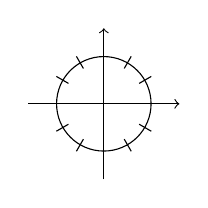
\begin{tikzpicture}[baseline=-0.6ex,scale=0.48]
  \draw[->] (-2.0,0)--(2.0,0);
  \draw[->] (0,-2.0)--(0,2.0);
  \draw (0,0) circle (1.25);
  \foreach \a in {0,30,...,330} {
    \draw ({1.08*cos(\a)},{1.08*sin(\a)}) -- ({1.45*cos(\a)},{1.45*sin(\a)});
  }
\end{tikzpicture}

\heading{Multiplication tables \ (finite groups)}

It can be viewed as the ID card of a finite group

It defines the structure of the group

It's an \((n\times n)\) array \((n\ \text{order of the group})\)

\[
\begin{array}{c|cccccc}
G & g_1 & g_2 & g_3 & \cdots & & g_n\\ \hline
g_1 & g_1^2 & g_1g_2 & g_1g_3 & \cdots & & g_1g_n\\
g_2 & g_2g_1 & g_2^2 & & & &\\
\vdots & & & \ddots & & &\\
g_n & & & & & & g_n^2
\end{array}
\]

\(\bigcirc\!\star\)\quad\heading{Rearrangement theorem}

Let us take any element of \(G\), \(g\)

Then composing (on the left or on the right) by \(g_0\) all the elements of \(G\)

We recover once and only once all the elements of \(G\), but in a different order

\arrowline implies that in the multiplication table in every row and in every column, each element must appear once.

\newpage

\heading{The symmetric group (or group of permutations) \(S_n\):}

\(S_n\) is the group of all permutations of an \(n\)-element set.

Let's denote \(p\), a permutation of \(n\) elements by
\[
p=\pmtx{1\quad 2\quad 3\quad\cdots\quad n}{p_1\quad p_2\quad p_3\quad\cdots\quad p_n}
=\pmtx{2\quad 5\quad 1\quad n\quad\cdots\quad 3}{p_2\quad p_5\quad p_1\quad p_n\quad\cdots\quad p_3}
\]

The composition of two permutations \(p\) and \(q\)
\[
\begin{aligned}
pq&=\pmtx{1\quad 2\quad\cdots\quad n}{p_1\quad p_2\quad\cdots\quad p_n}
\pmtx{1\quad 2\quad\cdots\quad n}{q_1\quad q_2\quad\cdots\quad q_n}\\
&=\pmtx{1\quad 2\quad\cdots\quad n}{p_1\quad p_2\quad\cdots\quad p_n}
\pmtx{p_1\quad p_2\quad\cdots\quad p_n}{q_{p_1}\quad q_{p_2}\quad\cdots\quad q_{p_n}}\\
&=\pmtx{1\quad 2\quad\cdots\quad n}{q_{p_1}\quad q_{p_2}\quad\cdots\quad q_{p_n}}
\end{aligned}
\]

\heading{Ex/ \(S_3\)}

\[
\begin{array}{c@{\qquad}c@{\qquad}c}
\pmtx{1&2&3}{1&2&3}=(e) &
\pmtx{1&2&3}{3&1&2}=(132) &
\pmtx{1&2&3}{2&3&1}=(123)\\[1.2em]
\pmtx{1&2&3}{1&3&2}=(23) &
\pmtx{1&2&3}{2&1&3}=(12) &
\pmtx{1&2&3}{3&2&1}=(13)
\end{array}
\]

\[
\textcolor{red}{S_3=\{(e),(12),(13),(23),(123),(132)\}}
\]

\begin{flushleft}
\(\bigstar\quad (132)(123)=
\pmtx{1&2&3}{3&1&2}
\pmtx{1&2&3}{2&3&1}
=
\pmtx{1&2&3}{3&1&2}
\pmtx{3&1&2}{1&2&3}
=
\pmtx{1&2&3}{1&2&3}=(e)\)

\begin{center}
\textcolor{red}{\large changed the columns}
\end{center}

\vspace{0.4em}
\(\bigstar\quad (12)(13)=
\pmtx{1&2&3}{2&1&3}
\pmtx{1&2&3}{3&2&1}\)

\begin{center}
\textcolor{gray}{\(\pmtx{1&2&3}{2&1&3}\pmtx{2&1&3}{3&2&1}
=\pmtx{1&2&3}{1&2&3}\)}
\end{center}

\begin{center}
\textcolor{green!45!black}{\large Swapping column leads to 1 wrong answer}

\textcolor{green!45!black}{(Sıralama sağdan değil tam tersi yapılmalı)}
\end{center}

\[
\begin{array}{rclclcl}
1&\longrightarrow^{(13)}&3&\longrightarrow^{(12)}&3\\[0.3em]
2&\longrightarrow^{(13)}&2&\longrightarrow^{(12)}&1\\[0.3em]
3&\longrightarrow^{(13)}&1&\longrightarrow^{(12)}&2
\end{array}
\qquad
=\pmtx{1&2&3}{3&1&2}=(132)
\]
\end{flushleft}

\end{document}
